\chapter{Event and candidate selection}
\label{chap:prod:sel}

The decay modes chosen for this analysis,
\DzToKpi, \DpToKpipi, \DspTophipi with \phiToKK, and \DstToDzpi with \DzToKpi, 
including their charge conjugates, are the amongst the most probable fully 
charged, hadronic final states for each meson.
The advantage of choosing such final states is that it allows the invariant 
mass of the charm hadrons to be computed unambiguously, so that a yield 
determination can be performed via fits to the mass distribution.
These fits shall be discussed in detail in \cref{chap:prod:fitting}, but it is 
worth noting at this point that such fits are simpler if the data is `clean', 
that is if the fraction of charm meson signal in the data is high.
It is then advantageous to optimise the selection of the data to reduce 
backgrounds, while retaining as much signal as possible to maximise the 
statistical significance of the measurement.

The selection of fully charged, hadronic decay modes of charm mesons has 
already been performed by many other analysis at \lhcb,\footnotemark and their 
selections share several common features.
The first of these is a requirement on the minimum charm candidate \pT, as 
there are many soft particles produced directly in the proton-proton collision, 
and such a requirement removes many of them.
The second is to ask that the charm candidate vertex is significantly displaced 
from the proton-proton collision vertex, or \ac{PV}, exploiting the long flight 
distances of charm hadrons in the laboratory frame.
Finally, it is required that the \ipchisq\ of the charm meson, a measure of the 
\acf{IP} relative to the uncertainty on the \ac{IP}, does not exceed a certain 
value.
This suppresses the background of charm candidates whose three-momentum does 
not point back to the \ac{PV}, which the momentum of random combinations of 
tracks will not, on average.
Each of these three features are powerful discriminators between signal and 
background.

\footnotetext{%
  Representative examples include selections of 
  \decay{\PDzero}{\PKmp\Ppipm}~\cite{Aaij:2012nva}, 
  \decay{\PDp}{\PKminus\PKplus\Ppiplus}~\cite{Aaij:2011cw}, and 
  \DspTophipi~\cite{Aaij:2012cy} decays.
}

For this measurement of prompt charm production it is preferable not to make 
\pT\ requirements on the charm candidate as they would restrict the \pT\ range 
available for differential measurements.
Nor is it desirable to make \ipchisq\ cuts, as the \ipchisq\ distribution is 
used for prompt-secondary discrimination, and having access to only part of the 
distribution can hinder accurate modelling.
The selection used is then informed by previous \lhcb\ studies of fully 
charged, hadronic charm decays, but with modifications to improve the 
usefulness for the measurement in hand.
The selection variables that are useful for discriminating between signal and 
background, in addition to those discussed, are given and described below.
The `parent' is the charm hadron \PHc, and the `children' are the charged 
hadrons in the final state.

\begin{description}
  \item[Child track \chisq\ per degree of freedom] \hfill \\
    The \chisq\ per degree of freedom of the child track returned by the track 
    fit.
    This variable discriminates between real and fake~(ghost) tracks.
  \item[Child transverse momentum] \hfill \\
    Momentum transverse to the $z$-axis.
    Children of charm hadrons will have a higher \pT\ on average than prompt 
    stable particles produced directly from the \pp\ collision.
  \item[Child momentum] \hfill \\
    Three-momentum magnitude \ptot.
    Must be within the range of acceptable particle identification performance 
    and fall within the kinematic spectrum of the \ac{PID} calibration samples, 
    discussed in \cref{chap:prod:effs:pid}.
  \item[Child pseudorapidity] \hfill \\
    Pseudorapidity \Eta, defined in \cref{eqn:intro:lhcb:pseudorapidity}.
    Must be within the range of acceptable particle identification performance 
    and fall within the kinematic spectrum of the \ac{PID} calibration samples.
  \item[Child \ipchisq] \hfill \\
    Impact parameter with respect to the \ac{PV}, as shown 
    in~\cref{fig:intro:lhcb:vertexing}.
    Prompt stable particles produced directly in the \pp\ collision will have a 
    low impact parameter, whereas particles produced in long-lived charm decays 
    will not have trajectories pointing back to the \ac{PV} on average.\\
    The `\chisq' is computed as $\Delta^{\text{T}}\Sigma^{-1}\Delta$, where 
    $\Delta$ is the difference in the position vectors of the track and the 
    vertex, and $\Sigma$ is the sum of the covariance matrices of the track and 
    vertex fits.
    This quantity is approximately equal to the ratio of the \ac{IP} and the 
    uncertainty on that \ac{IP} measurement.
  \item[Child \ac{PID}] \hfill \\
    Particle identification information as the combined response of the 
    calorimeters, muon stations, and \rich\ detectors.
    % TODO this will probably be explained in the detector chapter
    Predicted Cherenkov rings from tracks reconstructed by the tracking system 
    are compared with the photons detected by the {\rich}s.
    A global likelihood fit is then performed across all radiators and tracks, 
    and a likelihood, relative to the pion hypothesis, is assigned to each 
    track for each particle hypothesis.
  \item[Child pairwsie \ac{DOCA}] \hfill \\
    For a set of tracks physically originating from a common vertex, the 
    largest distance between any two tracks, the \ac{DOCA}, should be small.
  \item[Parent reconstructed mass] \hfill \\
    Invariant mass, either computed before the vertex fit as the sum of the 
    child four-momenta, or after as the mass of the fitted vertex.
    In a signal sample, a peaking structure will be seen around the nominal 
    charm hadron invariant mass.
    To be able to model the combinatorial background, the window around the 
    nominal mass should be many times wider than the resolution on this peak.
  \item[Parent vertex quality] \hfill \\
    Quality of the vertex fit.
    A larger \chisq\ value means a lower probability that the input tracks 
    originated from the same spatial point, which would be true if the tracks 
    were the product of a particle decay.
  \item[Parent vertex displacement] \hfill \\
    Displacement of the decay vertex from the production vertex, assumed to be 
    the \ac{PV}, as either the reconstructed lifetime $c\lifetime$ or the 
    vertex displacement \chisq.
    The `\chisq' is computed as $\Delta^{\text{T}}\Sigma^{-1}\Delta$, where 
    $\Delta$ is the difference in the spatial positions of the two vertices, and 
    $\Sigma$ is the sum of the covariance matrices of the two vertex fits.
  \item[Parent \ac{DIRA}] \hfill \\
    If the child tracks are from a true decay, and the decay vertex position is 
    correctly reconstructed, then the momentum vector of the parent should 
    point in the same direction as the displacement vector between the 
    production vertex and the decay vertex.
    The angle between the momentum and displacement vectors, the \ac{DIRA}, 
    should be small for a correctly reconstructed signal decay.
\end{description}

The exact numerical requirements made on these quantities were not tuned to 
optimise any specific figure of merit.
Instead, the values were chosen based on those used in previous charm analysis, 
generally being loosened to account for the higher rate available to charm 
triggers during the early measurements period, and the desire to have as high 
an efficiency as possible in the low \pT\ regions of the measurement.

As this analysis uses the Turbo stream, the only selection is `online', in that 
is performed on quantities computed in the trigger.
Still, the values computed are available `offline', once the data has been made 
available to analysts.
The selection is then split in two: the `online' part, which is the selection 
defined in the trigger and cannot be tuned once the data has been taken, and 
the `offline' selection, which is any selection made after this.
The use of the Turbo stream permits only one pass of the full event 
reconstruction, that done `online' in the trigger.
The following \namecref{chap:prod:sel:online} shall detail the online 
selection, and will be followed by a description of the offline selection shall 
follow in \cref{chap:prod:sel:offline}.

\section{Online selection and reconstruction}
\label{chap:prod:sel:online}

The different stages of the trigger are described in 
\cref{chap:intro:lhcb:detector:trigger}.
At \lzero, bunch-bunch crossings are accepted randomly by the \nobias\ trigger, 
so called because it should not bias any distributions of interest.
The rate at which the \nobias\ trigger accepts events is programmed into the 
hardware controller manually, with the exact rate depending on the number of 
colliding bunches at \lhcb.
The rates were tuned throughout the early measurements period so as to keep the 
detector `dead time' to a minimum.\footnotemark\
The \lzero\ rate is given for each fill in 
\cref{tab:prod:sel:online:l0_nobias_rateeff}.

\footnotetext{%
  The detector dead time is the period during which triggers by the \lzero\ are 
  `lost' due to the read-out buffer being full.
  The buffer is able to hold 16 events, each of which takes 40 \ac{LHC} clock 
  cycles, of \SI{25}{\nano\second} each, to be sent to the \hlt.
  Dead time can then occur if several triggers occur too close to one 
  another~\cite{Schmelling:1998qta}.
}

In \hltone, the following sequence is performed for events passing \lzero:
\begin{enumerate}
  \item The full offline charged particle (track) reconstruction is run for 
    hits inside the \velo\ sub-detector;
  \item The full offline \ac{PV} reconstruction is run, using as input only the 
    \velo\ tracks reconstructed in the previous step; and
  \item The reconstruction of `long' tracks, by first extrapolating \velo\ 
    tracks into the \ttracker\ and then, if at least two matching hits are 
    found in the \ttracker, extrapolating through the magnetic field.
    To decrease the time taken to assess all combinatorial combinations of 
    \velo+\ttracker\ tracks with hits in the \itracker\ and \otracker, only 
    hits within a search window assuming a \pT\ of at least \SI{800}{\MeVc} are 
    considered.
\end{enumerate}
Requiring all child tracks from a vertex to have $\pT > \SI{800}{\MeVc}$ would 
be inefficient for low \pT\ charm hadrons, and so the full decay is not 
reconstructed in \hltone.
Instead, the presence of a single, good quality track is required, which is 
consistent with having originated from a heavy flavour decay by having a large 
\ipchisq.
The full set of selection requirements is given in 
\cref{tab:prod:sel:online:hlt1_selection}.

\hlttwo\ performs the full, offline event reconstruction on events passing 
\hltone.
One \hlttwo\ selection, or `\hlttwo\ line', is defined per charm decay 
topology, corresponding to: one line for \DzToKpi; one line for the charged 
three-body decays, namely \DpToKpipi\ and \DspToKKpi; and one line for 
\DstToDzpi.
In the \PDzero, \PDplus, and \PDsplus lines, candidates are made by combining 
long tracks whose particle hypotheses are consistent with the final state under 
consideration.
In the \PDstarp\ line, \PDzero\ candidates passing the \PDzero\ \hlttwo\ line 
are combined with pion candidates, referred to here as `soft pions', 
\Ppiplussoft, due to their soft momentum distribution.
There are three stages to the particle combination: when cuts are applied to 
the input tracks; when cuts applied to the four-vector sum of these tracks; and 
when cuts are applied to the fitted vertex.
For computing efficiency, the combination does not proceed past a failing step, 
and combinations where the vertex fit fails to converge are discarded, although 
the likelihood of a failing vertex fit is suppressed by making \ac{DOCA} 
requirements beforehand.
The \DzToKpi, \DTohhh, and \DstToDzpi\ requirements are given in 
\cref{tab:prod:sel:online:hlt2_dztokpi_selection,tab:prod:sel:online:hlt2_dtohhh_selection,tab:prod:sel:online:hlt2_dsttodzpi_selection}.
Distributions of the charm candidate invariant mass after the full trigger 
selection are given in 
\cref{fig:prod:sel:D0ToKpi:online,fig:prod:sel:DpToKpipi:online,fig:prod:sel:DsToKKpi:online,fig:prod:sel:DstToD0pi_D0ToKpi:online}.

\begin{table}
  \caption{%
    List of fills used in analysis, along with the integrated luminosity 
    \intlumi, the \lzero\ \nobias\ rate, and the corresponding effective 
    \lzero\ efficiency (``eff.'') for each fill.
  }
  \label{tab:prod:sel:online:l0_nobias_rateeff}
  \centering
  \begin{tabular}{lS[table-figures-uncertainty=1]cS[table-format=2.2]}
  \toprule
  Fill number & {\intlumi (\si{\per\nb})} & \lzero\ \nobias\ rate (\si{\kilo\hertz}) & {\lzero\ \nobias\ eff. (\si{\percent})} \\
  \midrule
  3976        & 628 \pm 24                & 250                                      & 20.58                                   \\
  3981        & 1101 \pm 43               & 300                                      & 10.84                                   \\
  3988        & 931 \pm 36                & 300                                      & 10.84                                   \\
  3992        & 1310 \pm 51               & 350                                      & 7.84                                    \\
  3996        & 999 \pm 39                & 350                                      & 7.84                                    \\
  \bottomrule
\end{tabular}

\end{table}

\begin{table}
  \caption{%
    Requirements made on the track that fires the \hltone\ trigger line.
  }
  \label{tab:prod:sel:online:hlt1_selection}
  \centering
  \begin{tabular}{lcc}
  \toprule
  Particle                   & Variable     & Cut value          \\
  \midrule
  \multirow{5}{*}{Any track} & \pT          & $> \SI{800}{\MeV}$ \\
                             & \ptot        & $> \SI{3}{\GeV}$   \\
                             & Track \chisq & $< 3$              \\
                             & \ipchisq     & $> 10$             \\
                             & \velo\ hits  & $> 9$              \\
  \bottomrule
\end{tabular}

\end{table}

\begin{table}
  \caption{%
    Requirements made in the \hlttwo\ \DzToKpi\ selection.
    The track \chisq\ criterion is applied in the reconstruction and listed 
    here for completeness.
  }
  \label{tab:prod:sel:online:hlt2_dztokpi_selection}
  \centering
  \begin{tabular}{lccc}
  \toprule
  Particle                        & Variable                   &
  Cut value                      \\
  \midrule
  \multirow{4}{*}{\Ppipm, \PKpm}  & \pT                        & $> \SI{250}{\MeV}$                      \\
                                  & \ptot                      & $\ptot > \SI{2}{\GeV}$                  \\
                                  & Track \chisq               & $< 3$                                   \\
                                  & \ipchisq                   & $> 16$                                  \\
  \midrule
  \Ppipm                          & \dllkpi                    & $< 5$                                   \\
  \midrule
  \PKpm                           & \dllkpi                    & $> 5$                                   \\
  \midrule
  \multirow{5}{*}{\PDzero}        & $m(\PKminus\Ppiplus)$      & $\SI{1784}{\MeV} < m < \SI{1944}{\MeV}$ \\
                                  & \PK to \Ppi DOCA           & $< \SI{0.1}{mm}$                        \\
                                  & Vertex fit \chisq          & $< 10$                                  \\
                                  & Direction angle            & $< \SI{17}{\milli\radian}$              \\
                                  & Vertex displacement \chisq & $> 49$                                  \\
  \bottomrule
\end{tabular}

\end{table}

\begin{table}
  \caption{%
    Requirements made in the \hlttwo\ \DTohhh\ selection.
    The \PDp and \PDsplus candidates are defined according to the three-body 
    mass window after the vertex fit.
    Cuts of the form $x > x_{1},\, x_{2},\, x_{3}$ require that all particles 
    satisfy $x > x_{1}$, at least two satisfy $x > x_{2}$, and at least one 
    satisfies $x > x_{3}$.
    The track \chisq\ criterion is applied in the reconstruction and listed 
    here for completeness.
  }
  \label{tab:prod:sel:online:hlt2_dtohhh_selection}
  \centering
  \begin{tabular}{lccc}
  \toprule
  Particle                          & Variable                   & Cut value                                           \\
  \midrule
  \multirow{4}{*}{\Ppipm, \PKpm}    & \pT                        & $> 200,\, 400,\, \SI{1000}{\MeV}$                   \\
                                    & \ptot                      & $\ptot > \SI{2}{\GeV}$                              \\
                                    & Track \chisq               & $< 3$                                               \\
                                    & \ipchisq                   & $> 4,\, 10,\, 50$                                   \\
  \midrule
  \Ppipm                            & \dllkpi                    & $< 5$                                               \\
  \midrule
  \PKpm                             & \dllkpi                    & $> 5$                                               \\
  \midrule
  \PDplus                           & $m(\Phm\Php\Php)$          & $\SI{1789}{\MeV} < m < \SI{1949}{\MeV}$             \\
  \midrule
  \PDsplus                          & $m(\Phm\Php\Php)$          & $\SI{1889}{\MeV} < m < \SI{2049}{\MeV}$             \\
  \midrule
  \multirow{3}{*}{\PDplus/\PDsplus} & Vertex fit \chisq          & $< 25$                                              \\
                                    & Direction angle            & $< \SI{35}{\milli\radian}$                          \\
                                    & Vertex displacement \chisq & $> 16$ \text{AND} $\tau > \SI{0.150}{\pico\second}$ \\
  \bottomrule
\end{tabular}

\end{table}

\begin{table}
  \caption{%
    Requirements made in the \hlttwo\ \DstToDzpi\ selection.
    The input \PDzero\ candidates are those passing the \PDzero selection 
    defined in \cref{tab:prod:sel:online:hlt2_dztokpi_selection}.
    The track \chisq\ criterion is applied in the reconstruction and listed 
    here for completeness.
  }
  \label{tab:prod:sel:online:hlt2_dsttodzpi_selection}
  \centering
  \begin{tabular}{lccc}
  \toprule
  Particle                  & Variable                 & Cut value                             \\
  \midrule
  \multirow{2}{*}{\Ppipm}   & \pT                      & $> \SI{100}{\MeV}$                    \\
                            & Track \chisq             & $< 3$                                 \\
  \midrule
  \multirow{2}{*}{\PDstarp} & $m(\PDstarp)-m(\PDzero)$ & $\SI{130}{\MeV} < m < \SI{160}{\MeV}$ \\
                            & Vertex fit \chisq        & $< 25$                                \\
  \bottomrule
\end{tabular}

\end{table}

\section{Offline selection}
\label{chap:prod:sel:offline}

To improve the purity of the samples, the pion \ac{PID} requirement is 
tightened to $\dllkpi < 3$.
Furthermore, kinematic requirements are made on all \PDzero, \PDplus, and 
\PDsplus children such that they are within the fiducial region of phase space 
available for \ac{PID} efficiency calibration, which will be described in 
\cref{chap:prod:effs:pid}, specifically $3 < \ptot < \SI{100}{\GeVc}$ and $2 < 
\Eta < 5$.
As the three-body distributions still contain a large fraction of combinatorial 
background even after these additional cuts, the vertex fit \chisq\ and the 
direction angle cuts are tightened to $\chisq < 6$ and $\ac{DIRA} < 
\SI{14}{\milli\radian}$.

To reduce the combinatorial further for the \DspToKKpi\ mode, a requirement is 
made on the kaon pair as
\begin{equation}
  999.46 < m(\PKminus\PKplus) < \SI{1039.46}{\MeVcc}.
  \label{eqn:prod:sel:phi_cut}
\end{equation}
This corresponds to a $\pm\SI{20}{\MeVcc}$ window around the nominal mass of 
the $\phi(1020)$ meson~\cite{PDG2014}, which is referred to here as just 
`\Pphi'.
Around half of all \DspToKKpi\ decays proceed via the 
$\decay{\Pphi}{\PKminus\PKplus}$ channel~\cite{PDG2014}, and the narrow width 
of the \Pphi resonance makes this cut efficient at reducing the fraction of 
combinatorial background in the data, as well as reducing the fraction of $\Ppi 
\to \PK$ mis-identifications.
As the \DspToKKpi sample is then dominated by resonant \DspTophipi, the 
\PDsplus sample is referred as `\DspTophipi'.
The effective reduction of the total number of \PDsplus mesons produced due to 
the \Pphi requirement is treated as part of the branching fraction contribution 
in \cref{eqn:prod:introduction:differential_cross_section}, rather than as part 
of the selection efficiency.
The \DspTophipi\ branching fraction used is that given by the \cleo\ 
collaboration, where the same $\PKm\PKp$ mass window definition is 
used~\cite{Alexander:2008aa}.
The $\PKminus\PKplus$ mass spectrum from the \cleo\ measurement in shown in 
Figure~\ref{fig:sel:offline:cleo_phi}, along with the various mass windows with 
which they make several `\DspTophipi' branching fraction measurements, where 
the window corresponding to the measurement we use is delimited by solid red 
lines.

\begin{figure}
  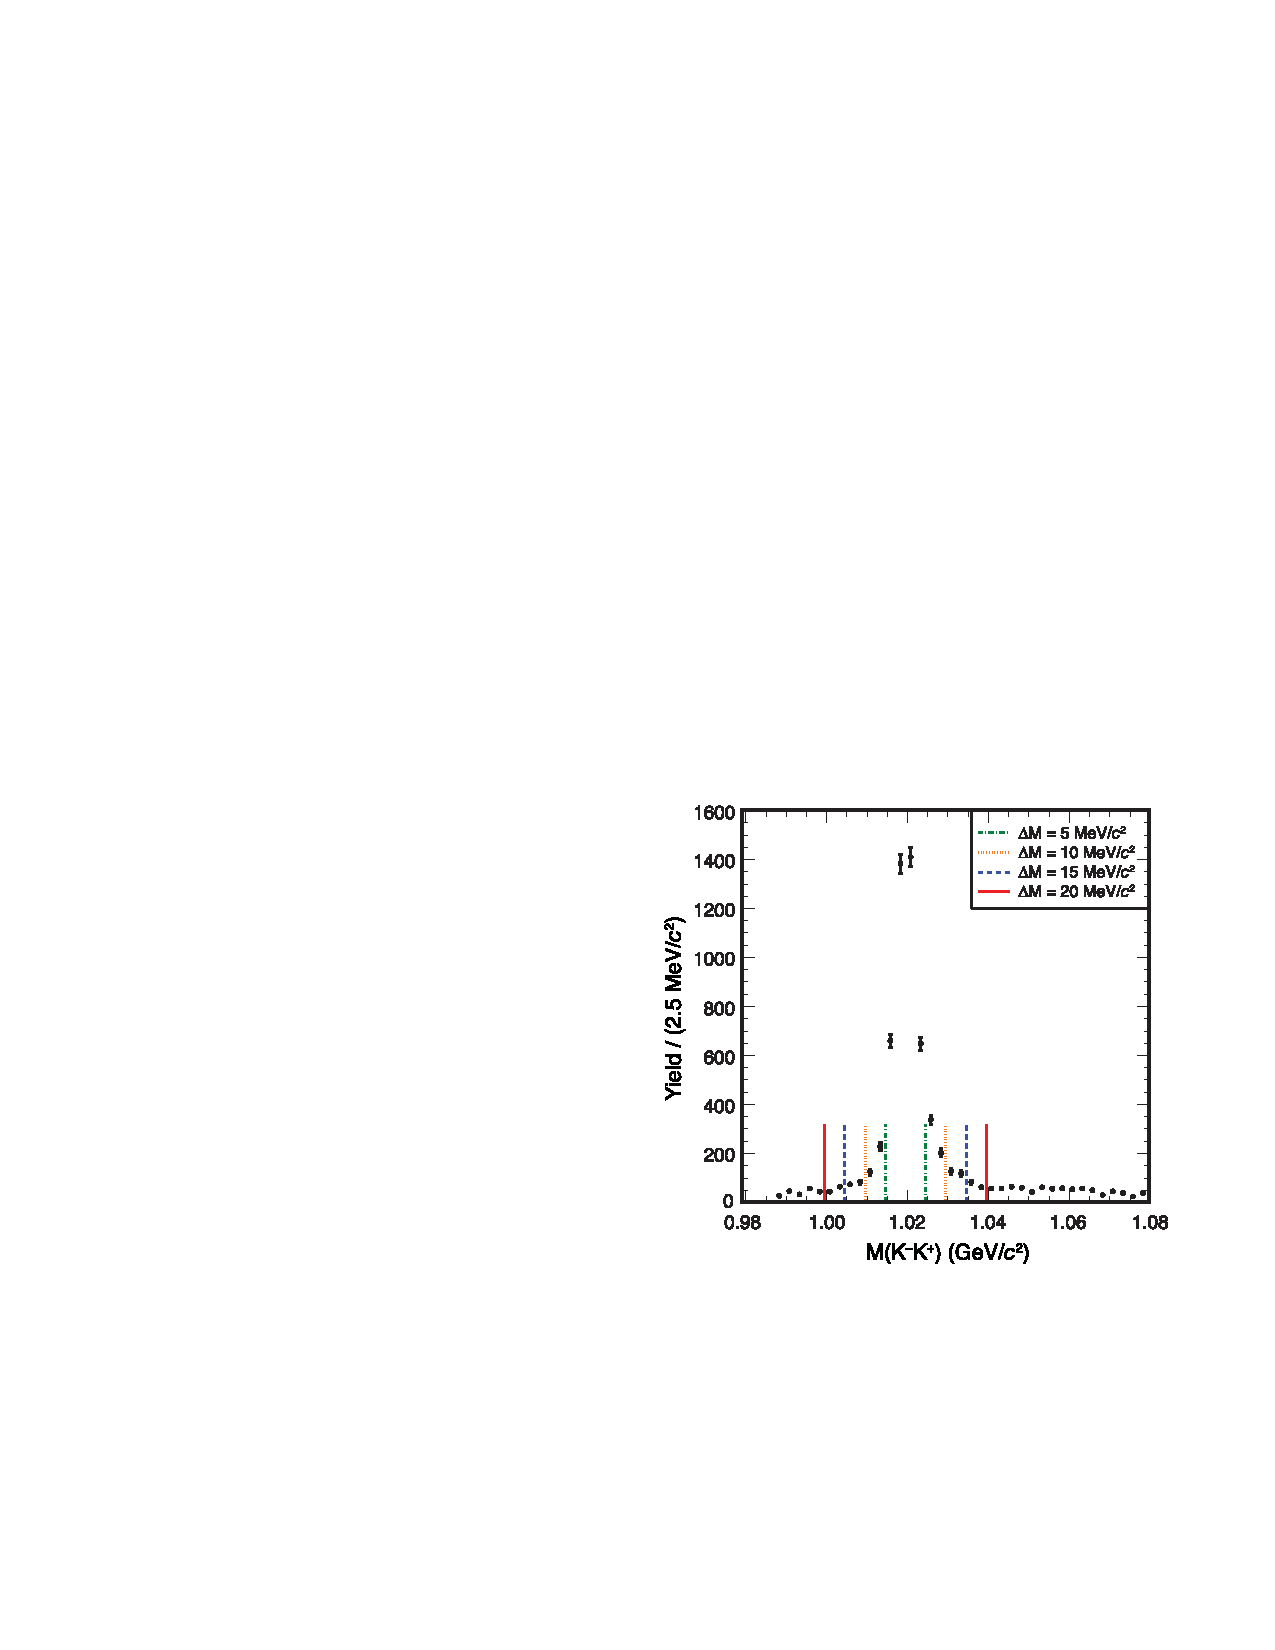
\includegraphics[width=\textwidth]{production/selection/cleo_phi_definition}
  \caption{%
    Definition of the $\PKminus\PKplus$ mass windows used by the \cleo\ 
    collaboration to measure the \DspTophipi branching 
    fraction~\cite{Alexander:2008aa}.
    The $\PKminus\PKplus$ mass window used in the charm production measurement 
    corresponds to the window delimited by the solid red lines in the figure.
  }
  \label{fig:sel:offline:cleo_phi}
\end{figure}

The charm candidate invariant mass distributions after the full offline 
selection after given in 
\cref{fig:prod:sel:D0ToKpi:offline,fig:prod:sel:DpToKpipi:offline,fig:prod:sel:DsToKKpi:offline,fig:prod:sel:DstToD0pi_D0ToKpi:offline}.
The number of charm candidates before and after the offline requirements are 
given in \cref{tab:prod:sel:candidates}.

\begin{figure}
  \begin{subfigure}[b]{0.5\textwidth}
    \centering
    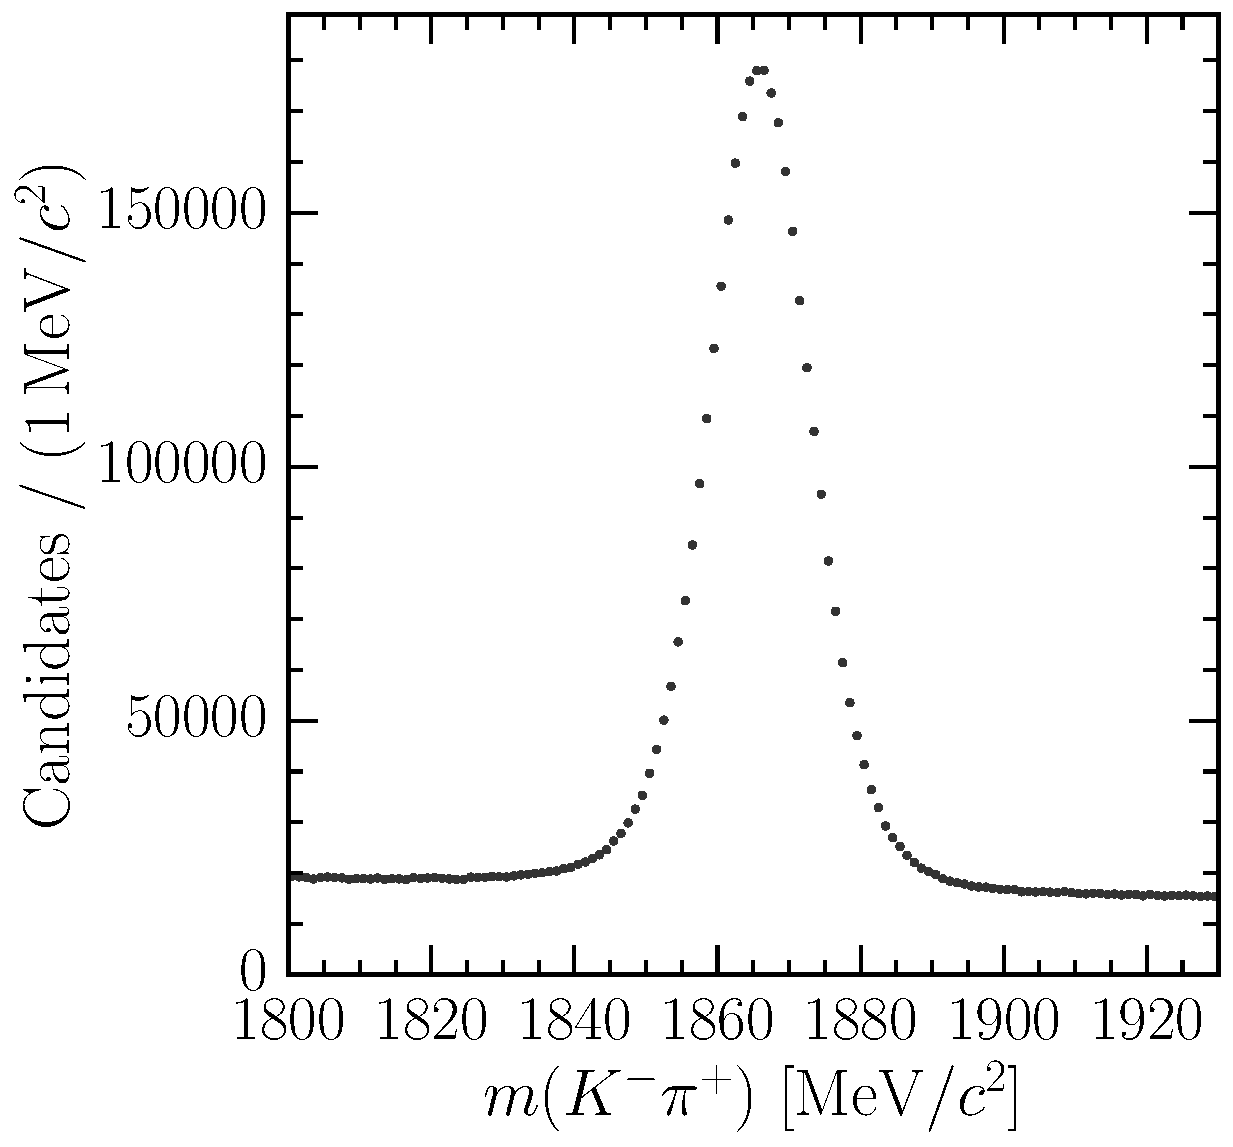
\includegraphics[width=\textwidth]{production/selection/D0ToKpi_mass}
    \caption{Online selected}
    \label{fig:prod:sel:D0ToKpi:online}
  \end{subfigure}
  \begin{subfigure}[b]{0.5\textwidth}
    \centering
    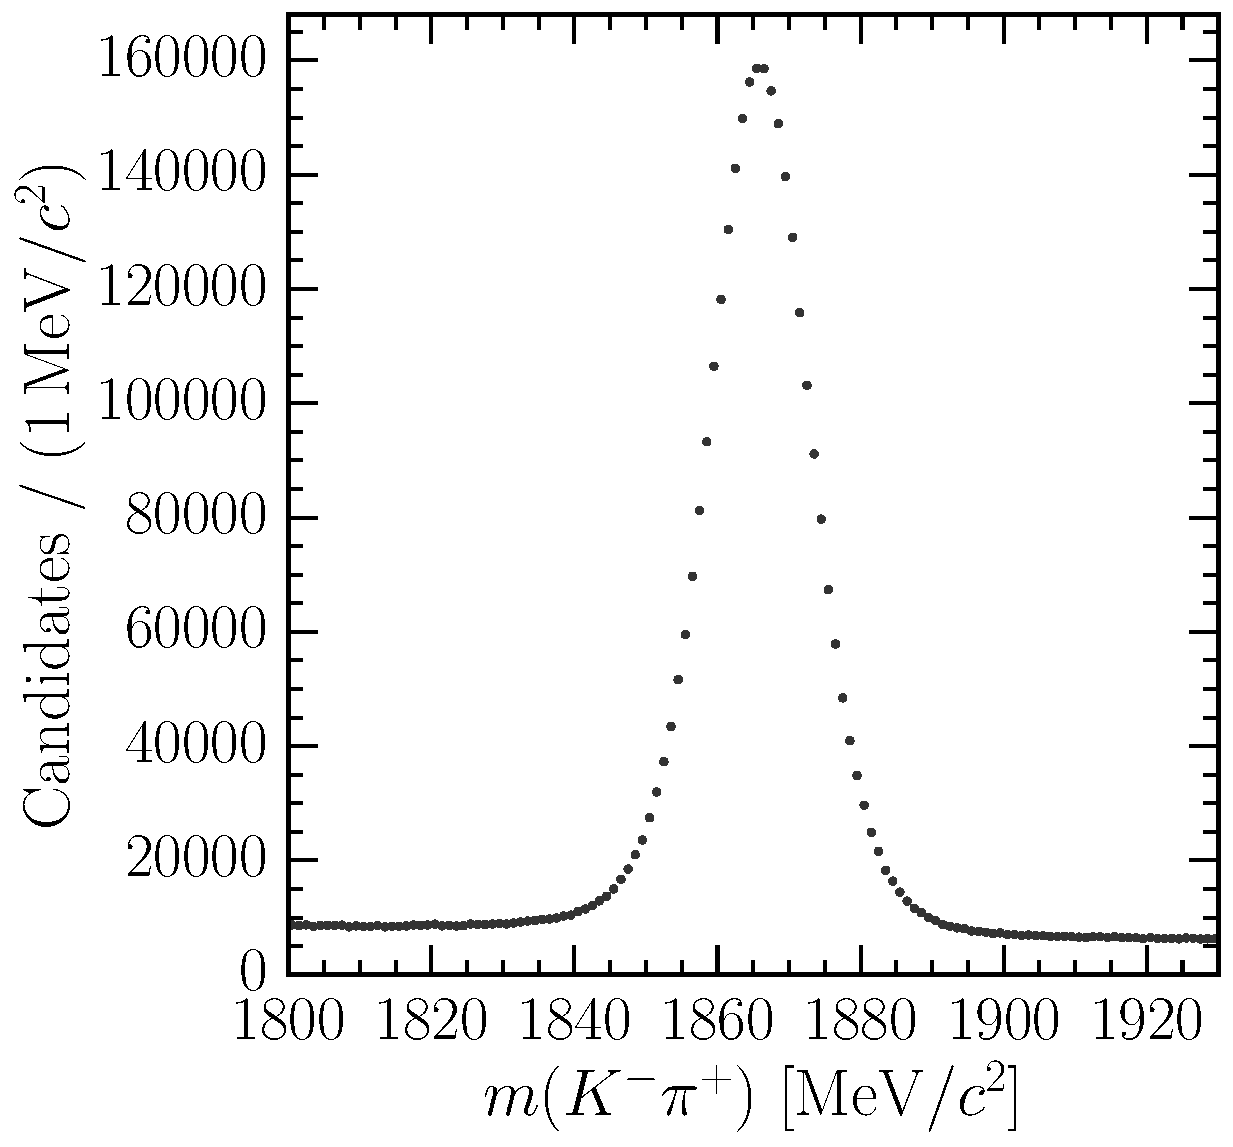
\includegraphics[width=\textwidth]{production/selection/D0ToKpi_mass_offline_selection}
    \caption{Offline selected}
    \label{fig:prod:sel:D0ToKpi:offline}
  \end{subfigure}
  \caption{%
    Mass distributions of \DzToKpi\ candidates after the online (trigger) 
    selection (\subref*{fig:prod:sel:D0ToKpi:online}) and after the offline 
    selection (\subref*{fig:prod:sel:D0ToKpi:offline}).
  }
  \label{fig:prod:sel:D0ToKpi}
\end{figure}

\begin{figure}
  \begin{subfigure}[b]{0.5\textwidth}
    \centering
    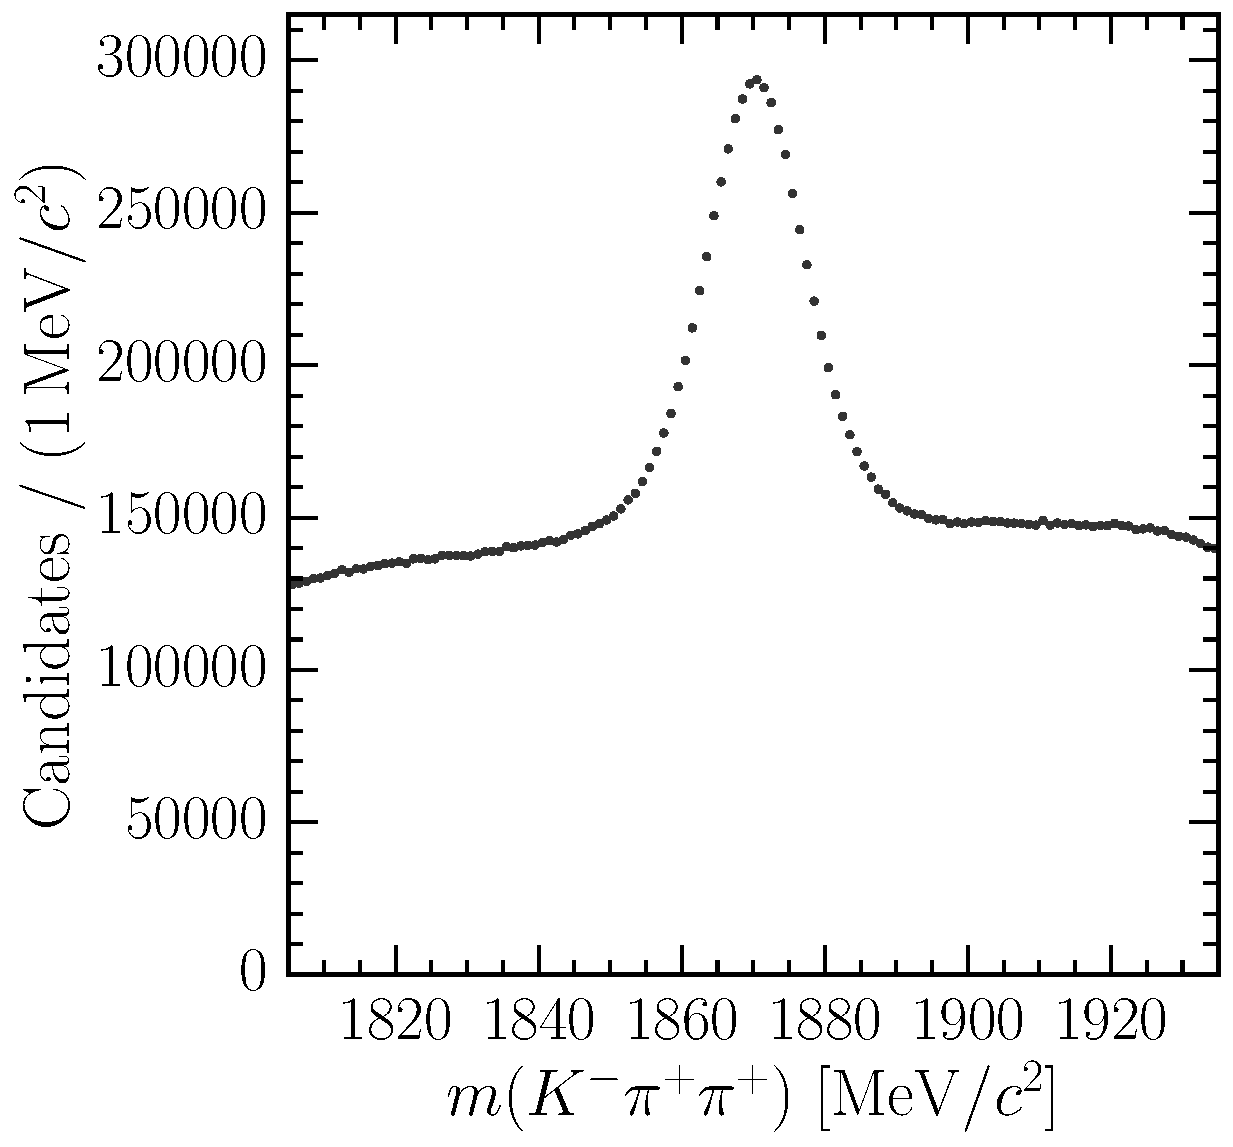
\includegraphics[width=\textwidth]{production/selection/DpToKpipi_mass}
    \caption{Online selected}
    \label{fig:prod:sel:DpToKpipi:online}
  \end{subfigure}
  \begin{subfigure}[b]{0.5\textwidth}
    \centering
    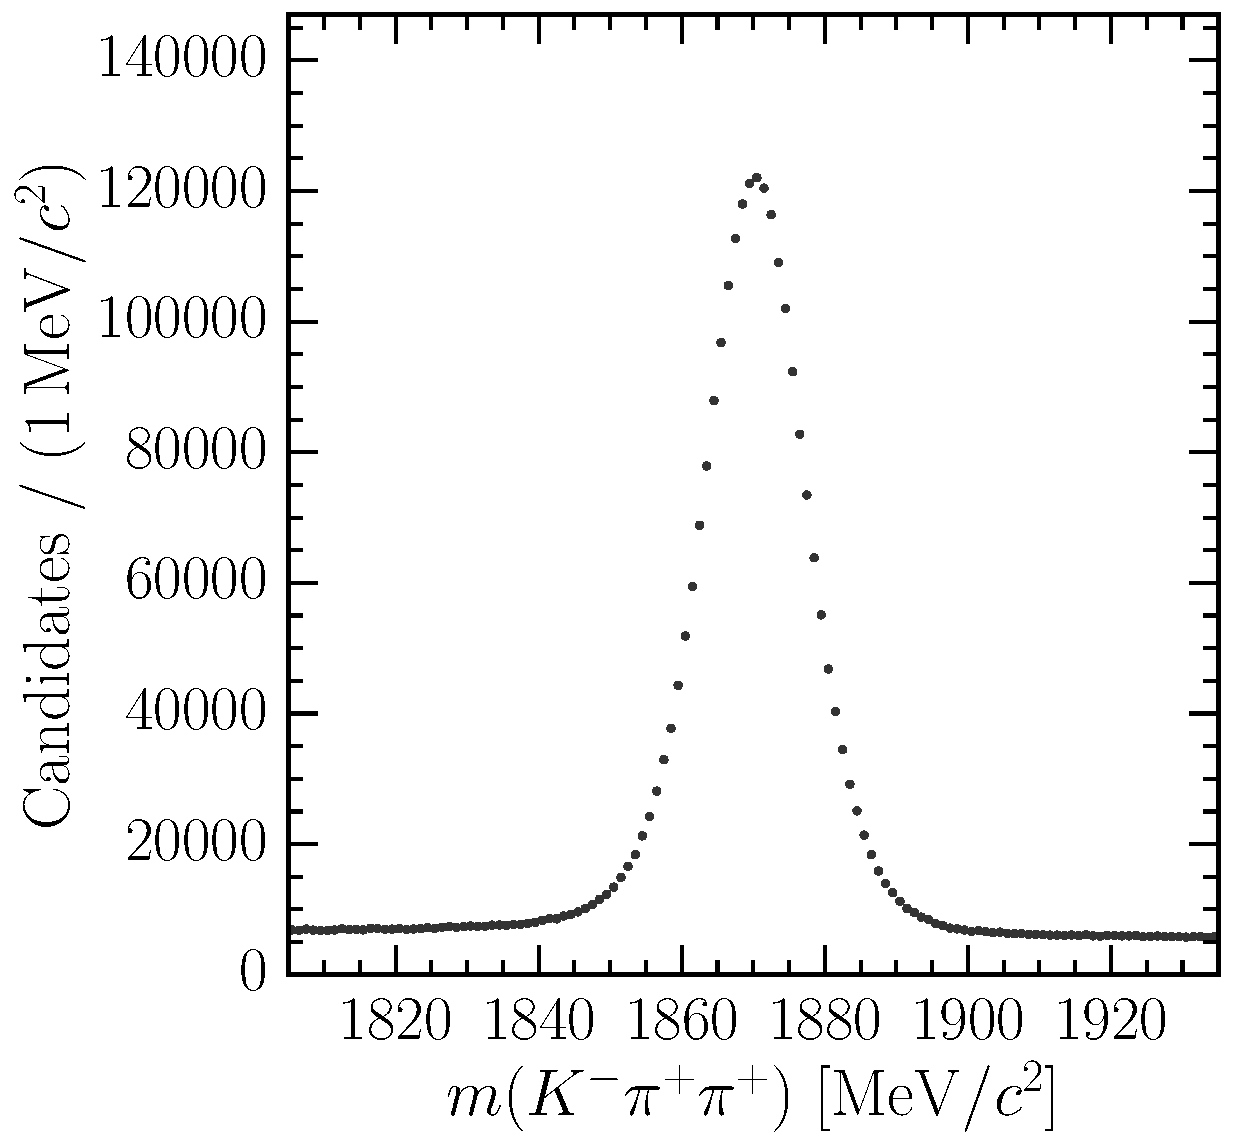
\includegraphics[width=\textwidth]{production/selection/DpToKpipi_mass_offline_selection}
    \caption{Offline selected}
    \label{fig:prod:sel:DpToKpipi:offline}
  \end{subfigure}
  \caption{%
    Mass distributions of \DpToKpipi\ candidates after the online (trigger) 
    selection (\subref*{fig:prod:sel:DpToKpipi:online}) and after the offline 
    selection (\subref*{fig:prod:sel:DpToKpipi:offline}).
  }
  \label{fig:prod:sel:DpToKpipi}
\end{figure}

\begin{figure}
  \begin{subfigure}[b]{0.5\textwidth}
    \centering
    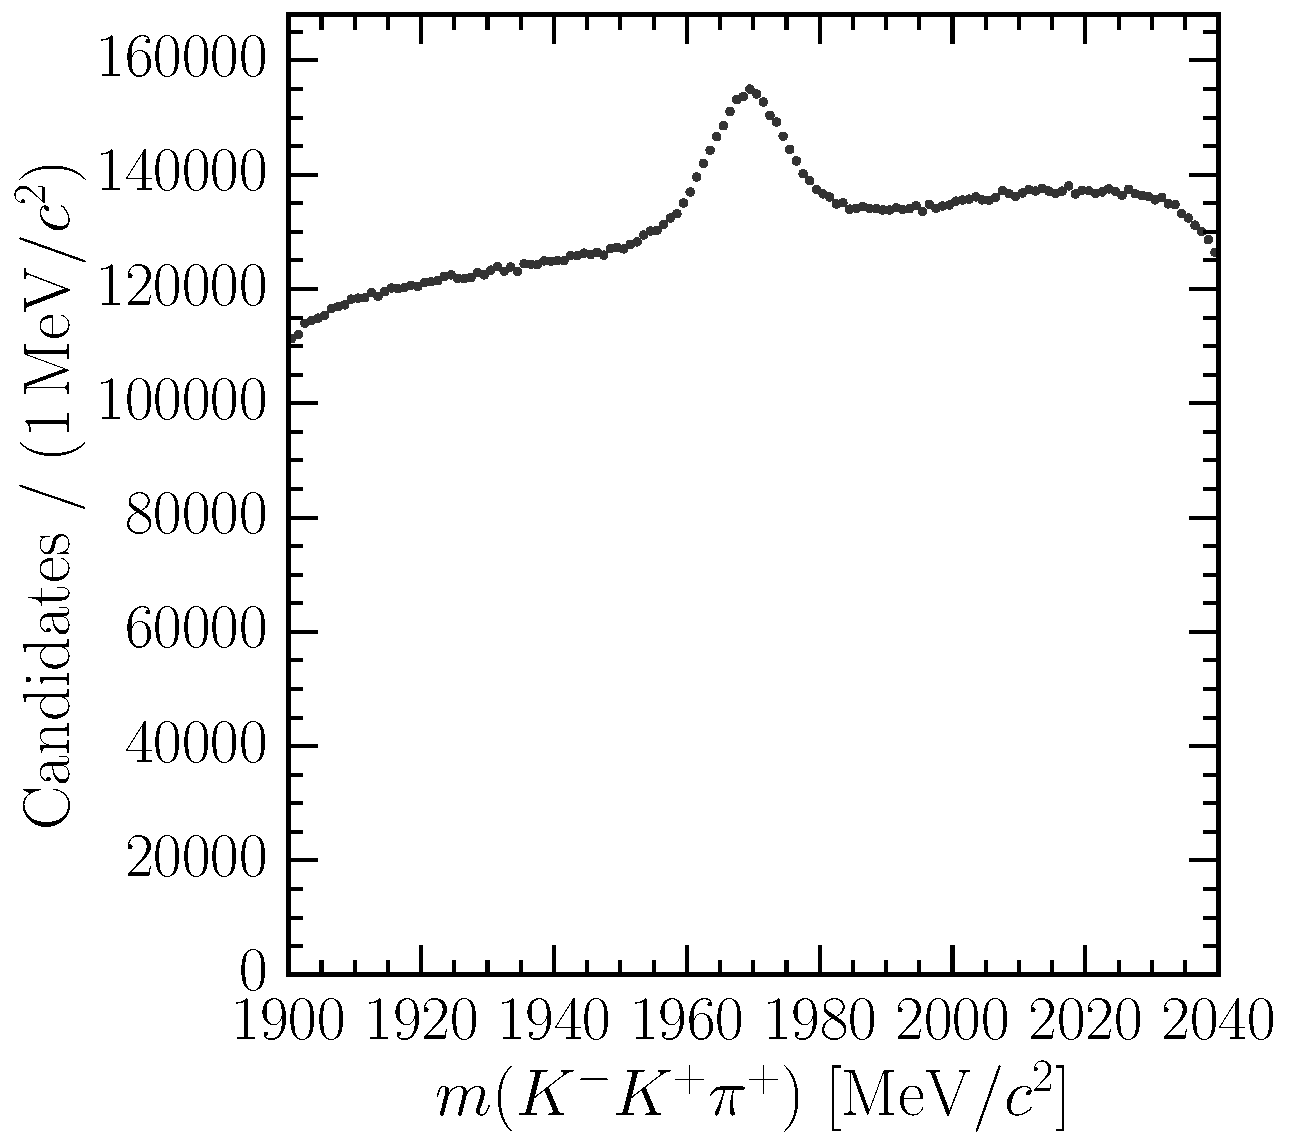
\includegraphics[width=\textwidth]{production/selection/DsToKKpi_mass}
    \caption{Online selected}
    \label{fig:prod:sel:DsToKKpi:online}
  \end{subfigure}
  \begin{subfigure}[b]{0.5\textwidth}
    \centering
    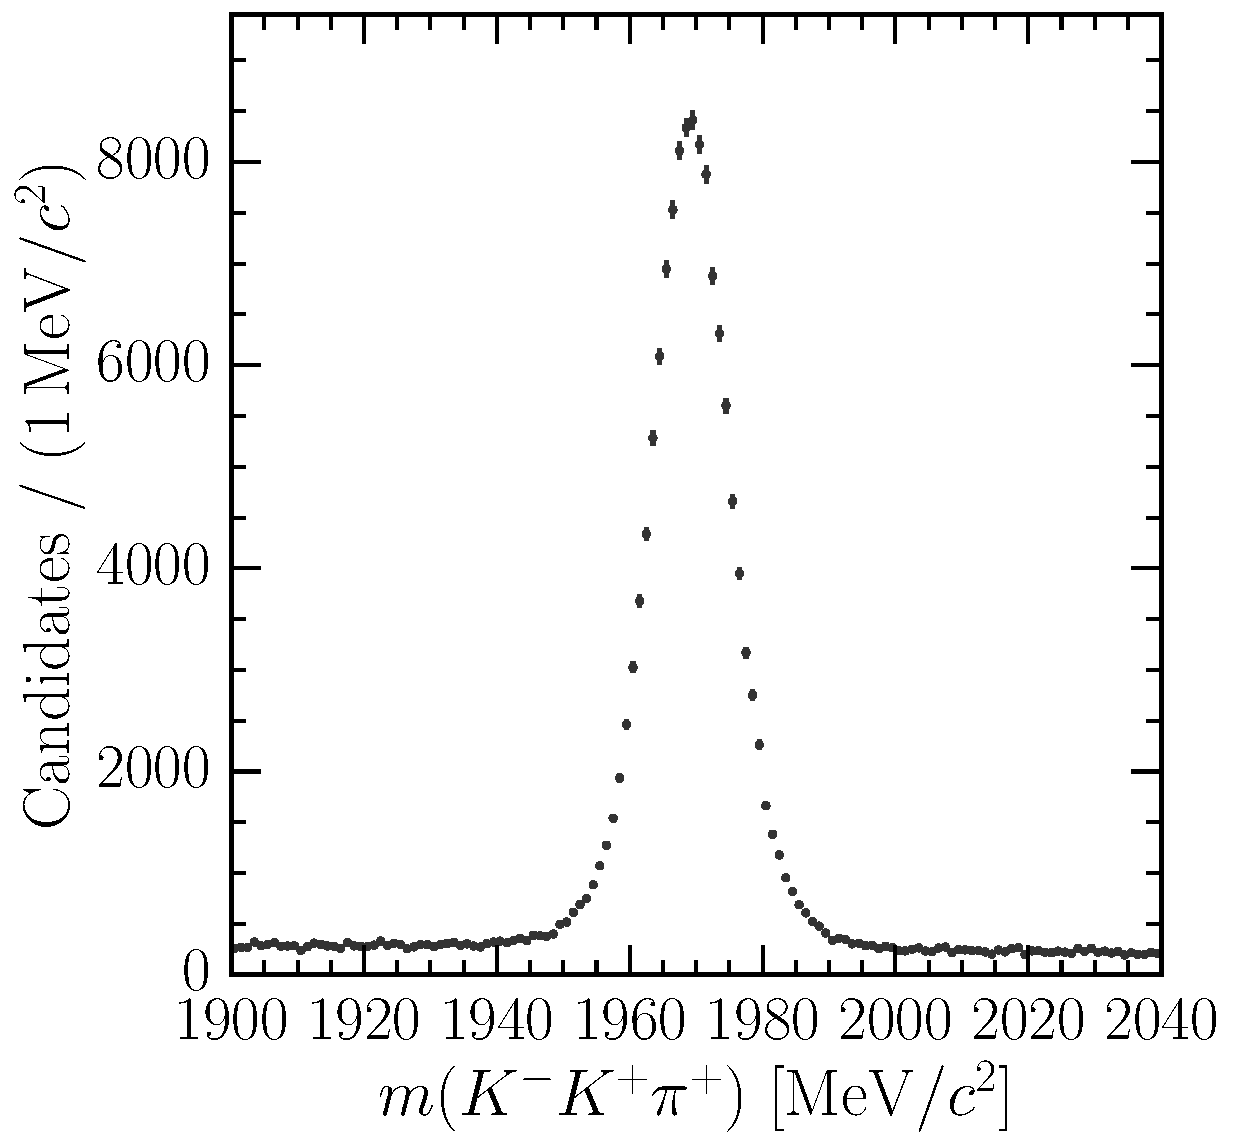
\includegraphics[width=\textwidth]{production/selection/DsToKKpi_mass_offline_selection}
    \caption{Offline selected}
    \label{fig:prod:sel:DsToKKpi:offline}
  \end{subfigure}
  \caption{%
    Mass distributions of \DspToKKpi\ candidates after the online (trigger) 
    selection (\subref*{fig:prod:sel:DsToKKpi:online}) and after the offline 
    selection (\subref*{fig:prod:sel:DsToKKpi:offline}).
    The offline selection includes the requirement that the kaon pair are 
    within a $\pm\SI{20}{\MeVcc}$ window around the nominal $\phi(1020)$ mass.
  }
  \label{fig:prod:sel:DsToKKpi}
\end{figure}

\begin{figure}
  \begin{subfigure}[b]{0.5\textwidth}
    \centering
    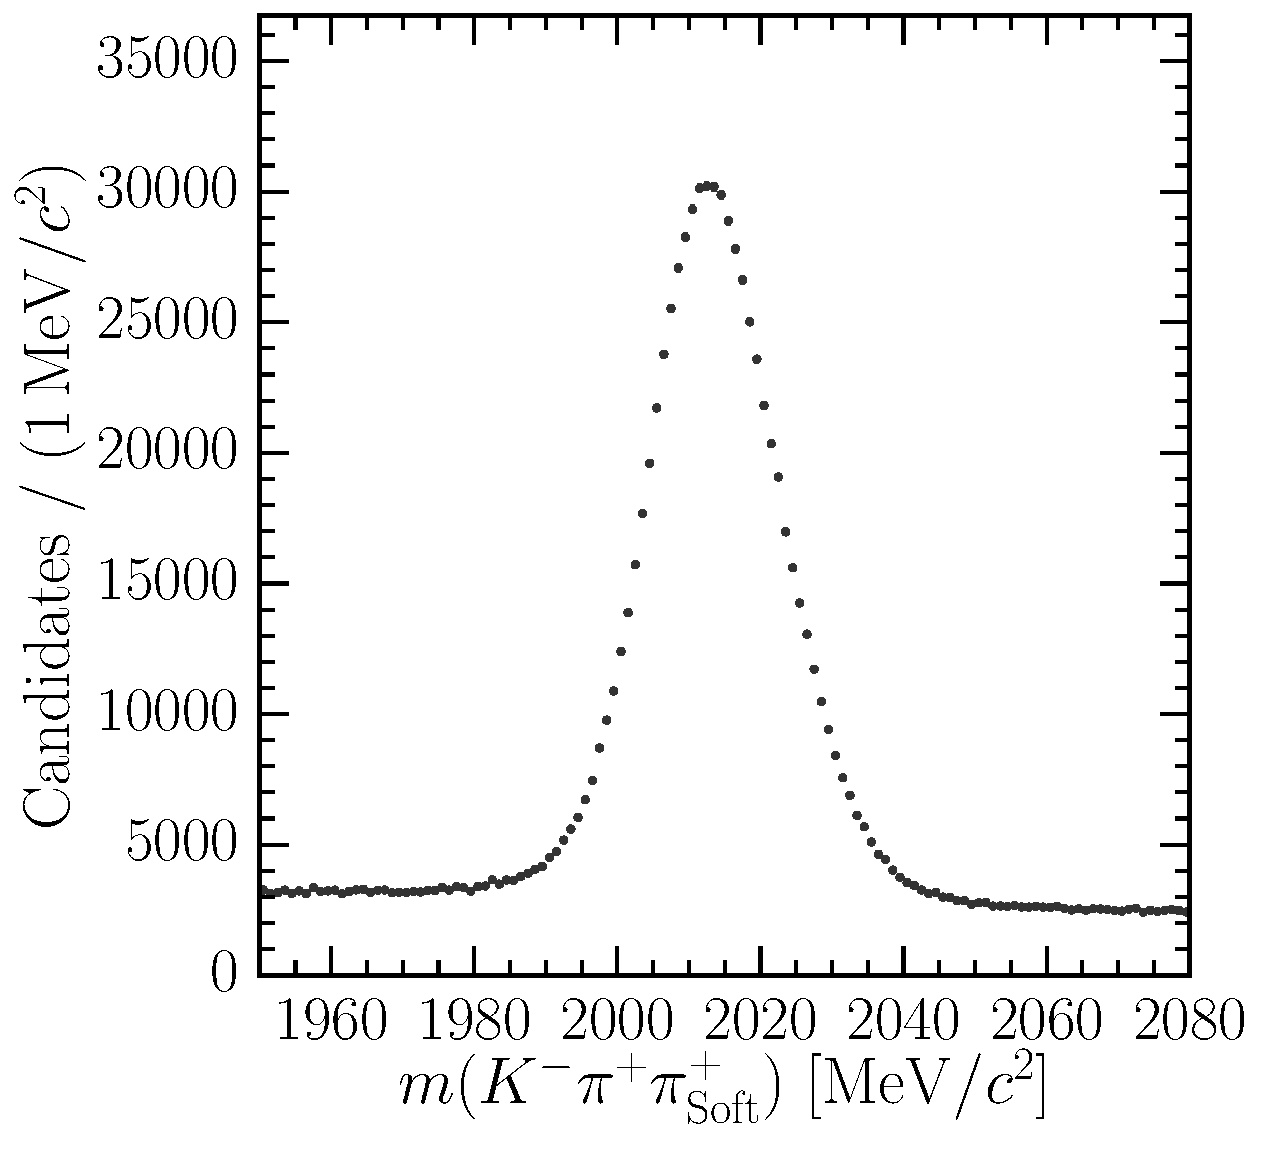
\includegraphics[width=\textwidth]{production/selection/DstToD0pi_D0ToKpi_mass}
    \caption{Online selected}
    \label{fig:prod:sel:DstToD0pi_D0ToKpi:online}
  \end{subfigure}
  \begin{subfigure}[b]{0.5\textwidth}
    \centering
    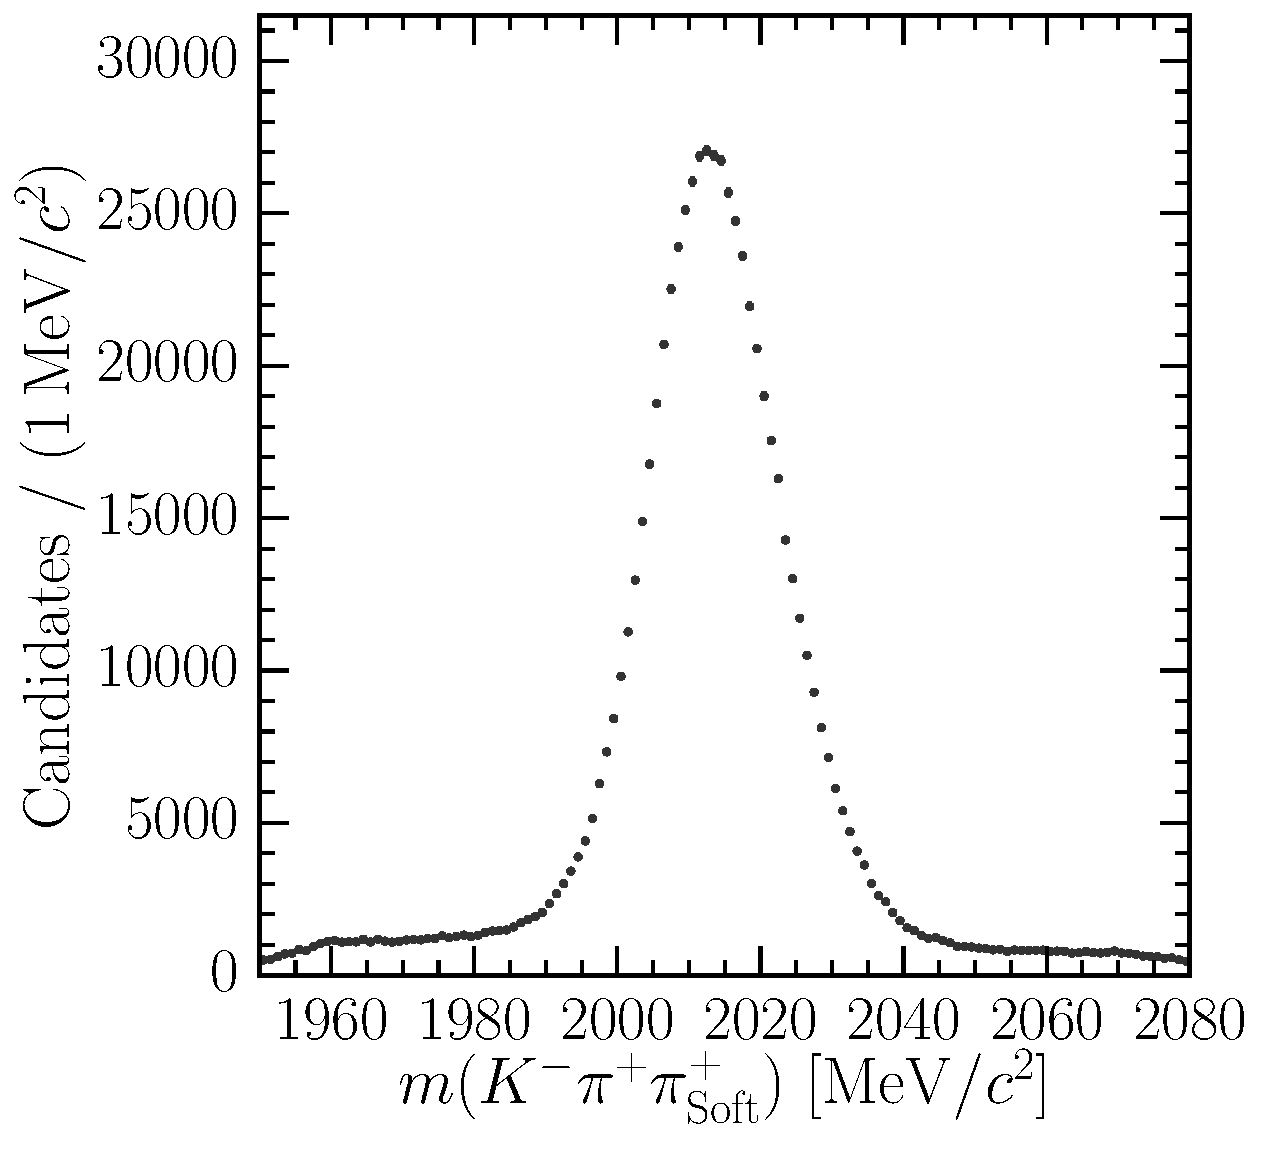
\includegraphics[width=\textwidth]{production/selection/DstToD0pi_D0ToKpi_mass_offline_selection}
    \caption{Offline selected}
    \label{fig:prod:sel:DstToD0pi_D0ToKpi:offline}
  \end{subfigure}
  \caption{%
    Mass distributions of \DstToDzpi\ candidates after the online (trigger) 
    selection (\subref*{fig:prod:sel:DstToD0pi_D0ToKpi:online}) and after the 
    offline selection (\subref*{fig:prod:sel:DstToD0pi_D0ToKpi:offline}).
  }
  \label{fig:prod:sel:DstToD0pi_D0ToKpi}
\end{figure}

\begin{table}
  \caption{%
    Number of candidates before and after the offline selection for each charm 
    candidate under study.
    The uncertainties given on the counts assuming Poisson statistics, and the 
    uncertainties given on the ratios assume binomial statistics.
  }
  \label{tab:prod:sel:candidates}
  \centering
  \begin{tabular}{lccc}
  \toprule
  Decay mode & {$N_{\text{Online}}$} [\num{e6}] & {$N_{\text{Offline}}$} [\num{e6}] & {$N_{\text{Offline}}/N_{\text{Online}}$ (\%)} \\
  \midrule
  \DzToKpi   & 5.8 & 3.8 & 65 \\
  \DpToKpipi & 25  & 3.1 & 12 \\
  \DspToKKpi & 21  & 0.16 & 0.8 \\
  \DstToDzpi & 1.1 & 0.72 & 66 \\
  \bottomrule
\end{tabular}

\end{table}
